\pagenumbering{arabic}
\documentclass[ucs]{beamer}
\usepackage{helvet}
\usepackage{eulervm}
%\usepackage[utf8x]{inputenc}
\usepackage{microtype}
\usepackage{calc}

\usepackage{tikz}
\usepgflibrary{shapes}
\usepgflibrary{arrows}

\usepackage{textcomp}
\makeatletter
\uc@dclc{8249}{default}{\textlangle}
\uc@dclc{8250}{default}{\textrangle}
\makeatother

\usepackage[compact]{fancyvrb1}
\DefineVerbatimEnvironment{code}{Verbatim}{commandchars=\\\{\}}

\def\>{\leavevmode\rlap{\color{blue}$\blacktriangleright$}\ \ }
\newcommand\slide[2]{#2<#1>}

\setbeamertemplate{section in toc}{{\leavevmode\llap{$\blacktriangleright$ }\bfseries\inserttocsection}\par}
\setbeamertemplate{section in toc shaded}{{\color{black}\inserttocsection}\par}
\setbeamertemplate{subsection in toc shaded}[default][50]

\AtBeginSection[]
{
  \begin{frame}<beamer>
    \frametitle{Outline}
    \tableofcontents[currentsection]
  \end{frame}
}

% To get the page numbers to stay constant on a frame [dpt]
\mode<presentation>
{
  \setbeamertemplate{sidebar left}{\thispdfpagelabel{\insertframenumber}}
}

\title{Finally tagless, partially evaluated}
\subtitle{Tagless staged interpreters for simpler typed languages}
\author{Jacques Carette and Oleg Kiselyov and Chung-chieh Shan}

\begin{document}

\newcommand{\authorstack}[3]{\begin{footnotesize}\begin{tabular}[t]{@{}c@{}}\begin{normalsize}#1\end{normalsize}\\[\jot]#2\\\texttt{#3}\end{tabular}\end{footnotesize}\ignorespaces}
\newsavebox\carette \sbox\carette{\authorstack{Jacques Carette}{McMaster University}{carette@mcmaster.ca}}
\newsavebox\oleg    \sbox\oleg   {\authorstack{Oleg Kiselyov}{FNMOC}{oleg@pobox.com}}
\newsavebox\ccshan  \sbox\ccshan {\authorstack{Chung-chieh Shan}{Rutgers University}{ccshan@rutgers.edu}}

\setbeamertemplate{sidebar right}{}

\author[Jacques Carette and Oleg Kiselyov and Chung-chieh Shan]{\usebox\carette \and \usebox\oleg \and \usebox\ccshan}
\date{APLAS\\30 November 2007}

\begin{frame}
    \titlepage
\end{frame}

\setbeamertemplate{background}{%
    \raisebox{0pt}[\paperheight][0pt]
        {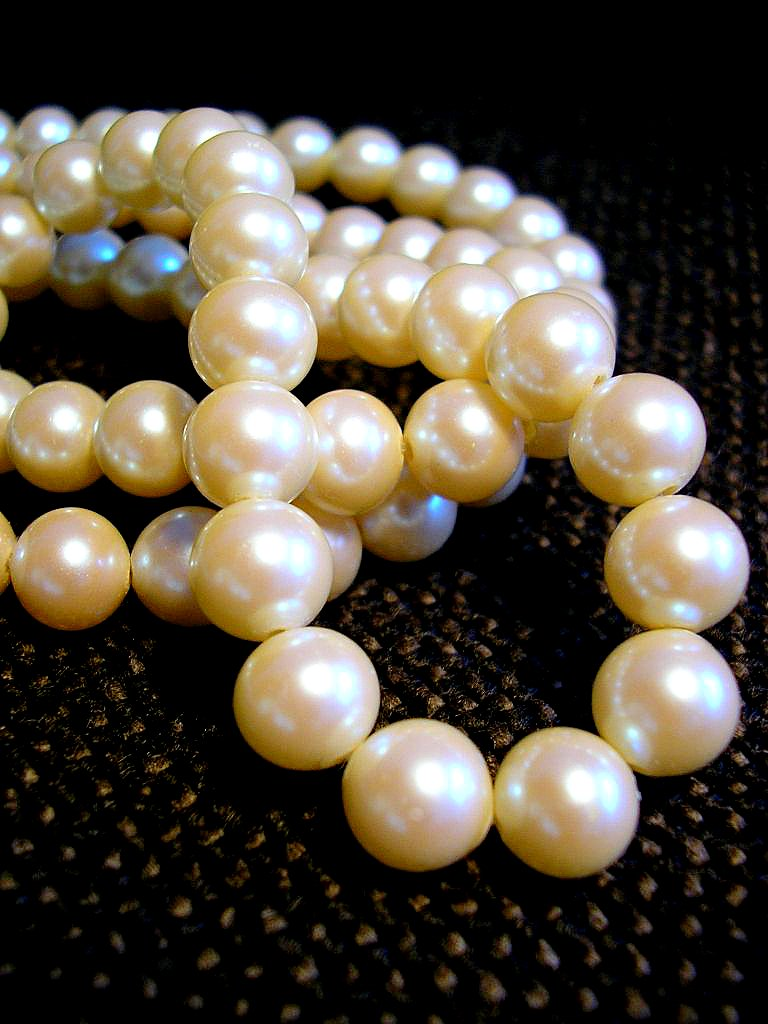
\includegraphics[width=\paperwidth+1pt,trim=0 100 0 0]{White_pearl_necklace.jpg}}%
    \llap{\href{http://www.flickr.com/photos/28481088@N00/160781390/}
               {\scriptsize\color{gray}tanakawho on flickr\kern1pt}}}
\begin{frame}
\end{frame}
\setbeamertemplate{background}[default]

\setbeamertemplate{sidebar right}{\vfill\llap{\usebeamerfont{framesubtitle}\insertframenumber\hskip\jot}\vskip\jot}

\tikzstyle{lang}=[ellipse,draw,anchor=west,text depth=3pt,text height=9pt]
\tikzstyle{every picture}=[>=angle 60]

\setbeamertemplate{background}{%
    \raisebox{0pt}[\paperheight][0pt]
        {
\includegraphics[width=\paperwidth,trim=0 35 0 180,clip]{FC0836213122.jpg}}}
\begin{frame}<1>[t,label=everywhere]{There's interpretation everywhere}
    A fold on an inductive data type is an interpreter of a domain-specific
    language.

    \bigskip
    \begin{tikzpicture}
        \draw node [lang] (lang0) {contract};
        \foreach \label/\prev/\cur in {grammar/0/1,music/1/2,$\lambda$-term/2/3}
            \draw (lang\prev.east)+(.3,0) node [lang] (lang\cur) {\label};
        \draw (lang3.east)+(.2,0) node [anchor=west] {\dots};
    \onslide<2>
        \draw (lang0)+(-110:2cm)   node (terp01) {value};
        \draw (lang0)+( -85:2.5cm) node (terp02) {schedule};
        \draw (lang1)+(-110:2cm)   node (terp11) {parse};
        \draw (lang1)+( -85:2.5cm) node (terp12) {pretty-print};
        \draw (lang2)+(-110:2cm)   node (terp21) {typeset};
        \draw (lang2)+( -85:2.5cm) node (terp22) {perform};
        \draw (lang3)+(-110:2cm)   node (terp31) {evaluate};
        \draw (lang3)+( -85:2.5cm) node (terp32) {compile};
        \foreach \lang in {0,...,3} {
            \draw (lang\lang)+(-65:1.5cm) node {\dots};
            \foreach \terp in {1,...,2}
                \draw [->] (lang\lang) -- (terp\lang\terp);
        }
    \onslide<3>
        \draw (lang3)+(-148:4.5cm)  node [inner xsep=0pt] (terp31) {evaluate};
        \draw (lang3)+(-133:4.25cm) node [inner xsep=0pt] (terp32) {compile};
        \draw (lang3)+(-113:4cm)    node [inner xsep=0pt] (terp33) {specialize};
        \draw (lang3)+( -93:4.4cm)  node [inner xsep=0pt] (terp34) {CPS transform};
        \draw (lang3)+( -73:4cm)    node [inner xsep=0pt] (terp35) {pretty-print};
        \draw (lang3)+( -58:3cm)    node {\dots};
        \foreach \terp in {1,...,5} \draw [->] (lang3) -- (terp3\terp);
    \end{tikzpicture}

    \only<2>{The same language can be interpreted in many useful ways.}%
    \only<3>{We focus on the $\lambda$-calculus as an example.}
\end{frame}
\setbeamertemplate{background}[default]
\againframe<2->[t]{everywhere}

\begin{frame}{Simple type preservation}
    \def\bool{\only<6-7>{\ \alert{bool}}}
    \begin{tikzpicture}
        \draw node [lang] (lang)
          {\texttt{\alt<7->{\onslide<7>{\alert{leq} (\alert{lit} 3, }%
                            \only<8>{\makebox[0pt]{\sffamily
                                      Simply typed $\lambda$-calculus}}%
                            \onslide<7>{\alert{lit} 4):}}
                           {\onslide<3->{LEQ (LIT 3, }%
                            \only<1>{\makebox[0pt]{\sffamily
                                      \alert{Typed} source language}}%
                            \only<2>{\makebox[0pt]{$3 \le 4$}}%
                            \onslide<3->{LIT 4):}}%
                   \makebox[3em][l]{\bool\only<3-6>{\ term}}}};
        \draw [->] (lang) --
            node [above,midway,anchor=east]
              {\only<1>{\alert{Typed} metalanguage\hspace*{2em}}%
               \only<2-3>{evaluate}%
               \only<8>{\begin{tabular}{@{}r@{\qquad}}
                        Haskell constructor instances\\
                        or ML functors
                        \end{tabular}}}
            node [above,midway,anchor=east,text width=2.5in,inner xsep=0pt]
                {\only<-3,8>{\color{bg}}\ttfamily
                \alt<7->{\only<7>{\alert<7>{lit:\ int -> int}\\
                lit i = i\\[1ex]
                \alert<7>{leq:\ int * int -> bool}\\
                leq (i,j) = i <= j}}
                {\only<3-6>{\alert<6>{eval:\ \only<6>{'a }term -> \only<6>{'a }value}\\
                eval (LIT i) = INT i\\
                eval (LEQ (m,n)) =\\
                \quad \alert<5>{match (eval m, eval n) with\\
                \quad (INT i, INT j) ->} BOOL (i <= j)}}}
            +(-100:4cm)
            node [anchor=north,text depth=0pt,text height=9pt]
              {\texttt{\llap{\onslide<3-6>{BOOL}
                             \onslide<3-7>{true:}%
                             \only<1>{\rlap{\sffamily
                                            \alert{Typed} target languages}}%
                             \only<2>{\rlap{\enspace$\mathsf{true}$}}%
                             \only<8>{\rlap{\sffamily evaluate}}}%
                       \makebox[3em][l]{\bool\only<3-6>{\ value}}}};
        \draw [->] (lang) -- +(-80:3.5cm)
            node [anchor=north west,inner xsep=0pt] {\only<8>{\hspace*{-16pt}compile}};
        \draw [->] (lang) -- +(-65:3cm)
            node [anchor=north west,inner xsep=0pt] {\only<8>{specialize}};
        \draw [->] (lang) -- +(-50:2.5cm)
            node [anchor=north west,inner xsep=0pt] {\only<8>{\hspace*{-3pt}CPS transform}};
        \draw      (lang)    +(-35:2cm) node {\dots};
    \end{tikzpicture}

    \bigskip

    \strut
    \only<-4>{It should be obvious in the metalanguage that interpreting
    a well-typed source term yields a well-typed target term.}%
    \only<5>{The term should be well-typed (and closed), so pattern matching
    in the metalanguage should always \textbf{obviously} succeed.}%
    \only<6>{Previous solutions use (and motivate) fancier types:\\
    generalized abstract data types, dependent types.}%
    \only<7>{Our simple solution is to be \textbf{finally tagless:}\\
    replace term constructors by cogen functions.}%
    \only<8>{The term accommodates \textbf{multiple interpretations}\\
    by abstracting over the cogen functions and their types.}%
    \strut
\end{frame}

\section{The object language}
\subsection{As a constructor class in Haskell}
\subsection{As a functor signature in ML}
\section{Tagless interpretation}
\subsection{Evaluation}
\subsection{Compilation}
\section{Type-indexed types}
\subsection{Partial evaluation}
\subsection{CPS transformation}

\begin{frame}{Conclusion}
    Initial type-checking can be done

    Preserves sharing
\end{frame}

\end{document}
